%%%%%%%%%%%%%%%%%%%%%%% file template.tex %%%%%%%%%%%%%%%%%%%%%%%%%
%
% This is a general template file for the LaTeX package SVJour3
% for Springer journals.          Springer Heidelberg 2010/09/16
%
% Copy it to a new file with a new name and use it as the basis
% for your article. Delete % signs as needed.
%
% This template includes a few options for different layouts and
% content for various journals. Please consult a previous issue of
% your journal as needed.
%
%%%%%%%%%%%%%%%%%%%%%%%%%%%%%%%%%%%%%%%%%%%%%%%%%%%%%%%%%%%%%%%%%%%
%
% First comes an example EPS file -- just ignore it and
% proceed on the \documentclass line
% your LaTeX will extract the file if required
\begin{filecontents*}{example.eps}
%!PS-Adobe-3.0 EPSF-3.0
%%BoundingBox: 19 19 221 221
%%CreationDate: Mon Sep 29 1997
%%Creator: programmed by hand (JK)
%%EndComments
gsave
newpath
  20 20 moveto
  20 220 lineto
  220 220 lineto
  220 20 lineto
closepath
2 setlinewidth
gsave
  .4 setgray fill
grestore
stroke
grestore
\end{filecontents*}
%
\RequirePackage{fix-cm}
%
%\documentclass{svjour3}                     % onecolumn (standard format)
%\documentclass[smallcondensed]{svjour3}     % onecolumn (ditto)
\documentclass[smallextended]{svjour3}       % onecolumn (second format)
%\documentclass[twocolumn]{svjour3}          % twocolumn
%
\smartqed  % flush right qed marks, e.g. at end of proof
%
\usepackage{amsmath}
\usepackage{xspace,stmaryrd,latexsym,url}
\usepackage{graphicx,tikz,rotating}
\usepackage[strings]{underscore}

%
% \usepackage{mathptmx}      % use Times fonts if available on your TeX system
%
% insert here the call for the packages your document requires
%\usepackage{latexsym}
% etc.
%
% please place your own definitions here and don't use \def but
% \newcommand{}{}
%
% Insert the name of "your journal" with
% \journalname{myjournal}
%


\def\D{\mathit{D}}
\def\E{\mathit{E}}

\def\FFOL{\mathit{FFOL}}
\def\V{\mathit{V}}
\def\F{\mathit{F}}
\def\P{\mathit{P}}
\def\True{\mathit{True}}
\def\False{\mathit{False}}
\def\Impl{\rightarrow}
\def\Descr{\rotatebox[origin=C]{180}{$\iota$}}
%\def\Descr{\rotate[c]{180}{\iota}}


% -----------------------------------------------

\def\lambdot{\rule{0.6mm}{0.6mm}\hspace{0.4ex}} 
\def\all#1{\forall #1\lambdot}
\def\exi#1{\exists #1\lambdot}
\def\lam#1{\lambda #1\lambdot}


\def\modal#1{#1}
\def\mfalse{\modal\bot}
\def\mtrue{\modal\top}
\def\mnot{\modal\neg\,}
\def\mor{\,\modal\vee\,}
\def\mand{\,\modal\wedge\,}
\def\mimpl{\,\modal\supset\,}
\def\miff{\,\modal\Leftrightarrow\,}
\def\mball#1{\modal\Box_{#1}\,}
\def\mdexi#1{\modal\Diamond_{#1}\,}
\def\mall#1{\modal{\forall}{#1}\lambdot\,}
\def\mexi#1{\modal{\exists}{#1}\lambdot\,}
\def\mpi{\modal{\Pi}\,}
\def\mvalid{\modal{\texttt{valid}}} 

\def\Metaeq{=}
\def\bnormform#1{\left.#1\hspace*{-.4ex}\right\downarrow_\beta}
\def\benormform#1{\left.#1\hspace*{-.4ex}\right\downarrow_{\beta\eta}}
\def\Bnormform#1{\left.{#1}\hspace*{-.4ex}\right\downarrow_\beta}
\def\Benormform#1{\left.{#1}\hspace*{-.4ex}\right\downarrow_{\beta\eta}}
\def\ambnormform#1{{#1}\hspace*{-1.1ex}\downarrow_{\kern-.2em\scriptscriptstyle *}} % ``ambiguous'' normal form
\def\eqb{\Metaeq_{\beta}}
\def\eqe{\Metaeq_{\eta}}
\def\eqbe{\Metaeq_{\beta\eta}}
\def\convarrow{\rightarrow}


\newcommand\entity[1]{\text{\textrm{#1}}}
\def\QHL{\entity{QHL}}
\def\QML{\entity{QML}}
\def\NOM{\entity{NOM}}
\def\SVAR{\entity{SVAR}}
\def\CON{\entity{CON}}
\def\FVAR{\entity{FVAR}}
%\def\IC{\entity{IC}}
\def\FSYM{\entity{FSYM}}
\def\RSYM{\entity{RSYM}}
\def\QHLSTT{\entity{QHLSTT}}
\def\QMLSTT{\entity{QMLSTT}}
\def\IV{\entity{IV}}
\def\PV{\entity{PV}}
\def\SYM{\entity{SYM}}
\def\IVSTT{\entity{IVSTT}}
\def\PVSTT{\entity{PVSTT}}
\def\SYMSTT{\entity{SYMSTT}}
\def\SSTT{\entity{SSTT}}
\def\AR{\entity{AR}}
\def\STT{\entity{STT}\xspace}

\def\QKPIm{\entity{QK}\pi^-\xspace}
\def\QKPI{\entity{QK}\pi\xspace}
\def\QKPIp{\entity{QK}\pi^+\xspace}
\def\QSFPIm{\entity{QS5}\pi^-\xspace}
\def\QSFPI{\entity{QS5}\pi\xspace}
\def\QSFPIp{\entity{QS5}\pi^+\xspace}

\def\stt{\entity{STT}\xspace}
\def\tt{\entity{STT}}
\def\lm{\entity{MM}\xspace}
\def\ipl{\entity{IPL}\xspace}
\def\HOML{\entity{HOML}\xspace}
\def\HOL{\entity{HOL}\xspace}

\def\worldtype{\mu}
\def\indtype{\iota}
\def\mutype{\mu}
\def\boola{\omicron}
\def\boolb{\hat{\omicron}}

\def\ar{\shortrightarrow}

\newcommand\map[1]{\hat{#1}}
\newcommand\hol[1]{\boldsymbol{#1}}
\newcommand\lift[1]{\lceil #1 \rceil}
\newcommand\llift[1]{\dot{#1}}

\newcommand{\imp}{\longrightarrow}
\newcommand{\limp}{\longleftarrow}
\newcommand{\biimp}{\longleftrightarrow}
\newcommand{\allq}{\forall}
\newcommand{\exq}{\exists}
\newcommand{\seq}{\vdash}
\newcommand{\nec}{\Box} % necessarily
\newcommand{\pos}{\Diamond} % possibly
\newcommand{\ess}[2]{#1 \ \mathit{ess.} \ #2}
\newcommand{\NE}{\mathit{NE}}


\def\ti{i}
\def\dom{\textit{dom \/}}
\def\cod{\textit{cod \/}}
\def\comp{\cdot}
\def\kleq{\cong}
\def\exid{\simeq}
\def\ddef{:=}
\def\id{\textit{I\/}}
\def\ex{\E}


\begin{document}

\title{Automating Free Logic in HOL, with an Application in Category Theory\thanks{Mention DFG grants ...}}
%\title{Free Logic and Axiom Systems for Category Theory in HOL\thanks{Mention DFG grants ...}}
%\title{Embedding Free Logic and Axiom Systems for Category Theory in HOL\thanks{Mention DFG grants ...}}
%\subtitle{(And an Exemplary Application in Category Theory)}

%\titlerunning{Short form of title}        % if too long for running head

\author{Christoph Benzm\"uller       \and
      Dana Scott 
}

%\authorrunning{Short form of author list} % if too long for running head

\institute{F. Author \at
              first address \\
              Tel.: +123-45-678910\\
              Fax: +123-45-678910\\
              \email{fauthor@example.com}           %  \\
%             \emph{Present address:} of F. Author  %  if needed
           \and
           S. Author \at
              second address
}

\date{Received: date / Accepted: date}
% The correct dates will be entered by the editor


\maketitle

\begin{abstract}
  % Partiality and undefinedness are prominent challenges in various
  % areas of mathematics and computer science.  Unfortunately, however,
  % modern proof assistant system based on traditional classical or
  % intuitionistic logics provide rather inadequate support for these
  % challenge concepts.  Free logic offers a theoretically appealing
  % solution, but is has been considered as rather unsuited towards
  % practical utilisation.

  % The two main contributions of this article are: (i) A shallow
  % semantical embedding of free logic in classical higher-order logic
  % is presented; this embedding enables the application of higher-order
  % interactive and automated theorem provers (and their integrated
  % subprovers) for the formalisation and verification of free logic
  % theories.  (ii) This approach to automate free logic is exemplarily
  % employed in a selected domain of mathematics: Starting from a
  % generalization of the standard axioms for a monoid we present a
  % stepwise development of various, mutually equivalent foundational
  % axiom systems for category theory. As a side-effect of this work
  % some (minor) issue in a prominent category theory textbook have been
  % revealed.

  A shallow semantical embedding of free logic in classical
  higher-order logic is presented, which enables the off-the-shelf
  application of higher-order interactive and automated theorem
  provers (and their integrated subprovers) for the formalisation and
  verification of free logic theories.  
  Subsequently, this approach is exemplarily employed in a selected domain of
  mathematics: starting from a generalization of the standard axioms
  for a monoid we present a stepwise development of various, mutually
  equivalent foundational axiom systems for category theory. As a
  side-effect of this work some (minor) issue in a prominent category
  theory textbook has been revealed.

  The purpose of this article is not to claim any novel results in
  category theory, but to demonstrate an elegant way to ``implement''
  and utilise interactive and automated reasoning in free logic, and
  to present respective experiments.


\keywords{Free Logic \and Classical Higher-Order Logic \and Category
  Theory \and Interactive and Automated Theorem Proving }
% \PACS{PACS code1 \and PACS code2 \and more}
% \subclass{MSC code1 \and MSC code2 \and more}
\end{abstract}

\section{Introduction}
\label{intro}
Partiality and undefinedness are prominent challenges in various areas
of mathematics and computer science.  Unfortunately, however, modern
proof assistant systems and automated theorem provers based on
traditional classical or intuitionistic logics provide rather
inadequate support for these challenge concepts.  Free logic offers a
theoretically appealing solution, but is has been considered as rather
unsuited towards practical utilisation.


In the first part of this article (\S2 and \S3) we show how free logic
can be elegantly ``implemented'' in any theorem proving system for
classical higher-order logic (HOL) \cite{B5}. The proposed solution
employs a semantic embedding of free (or inclusive logic) in HOL. We
present an exemplary implementation of this idea in the mathematical
proof assistant Isabelle/HOL \cite{NPW02}. Various state-of-the-art
first-order and higher-order automated theorem provers and model
finders are integrated (modulo suitable logic translations) with
Isabelle via the Sledgehammer tool \cite{Sledgehammer}, so that our
solution can be utilized, via Isabelle as foreground system, with a
whole range of other background reasoners. As a result we obtain an
elegant and powerful implementation of an interactive and automated
theorem proving (and model finding) system for free logic.


%   The two main contributions of this article are: (i) A shallow
%   semantical embedding of free logic in classical higher-order logic
%   is presented; this embedding enables the application of higher-order
%   interactive and automated theorem provers (and their integrated
%   subprovers) for the formalisation and verification of free logic
%   theories.  (ii) This approach to automate free logic is exemplarily
%   employed in a selected domain of mathematics: Starting from a
%   generalization of the standard axioms for a monoid we present a
%   stepwise development of various, mutually equivalent foundational
%   axiom systems for category theory. As a side-effect of this work
%   some (minor) issue in a prominent category theory textbook have been
%   revealed.



% Partiality and undefinedness are core concepts in various areas of
% mathematics.  Modern mathematical proof assistants and theorem proving
% systems are often based on traditional classical or intuitionistic
% logics and provide rather inadequate support for these challenge
% concepts.  Free logic @{cite "sep-logic-free,scott67:exist"}, in
% contrast, offers a theoretically and practically appealing
% solution. Unfortunately, however, we are not aware of any implemented
% and available theorem proving system for free logic.
 
% In this extended abstract we show how free logic can be
% ``implemented'' in any theorem proving system for classical
% higher-order logic (HOL) @{cite "B5"}. The proposed solution employs a
% semantic embedding of free (or inclusive logic) in HOL. We present an
% exemplary implementation of this idea in the mathematical proof
% assistant Isabelle/HOL @{cite "NPW02"}. Various state-of-the-art
% first-order and higher-order automated theorem provers and model
% finders are integrated (modulo suitable logic translations) with
% Isabelle via the Sledgehammer tool @{cite "Sledgehammer"}, so that our
% solution can be utilized, via Isabelle as foreground system, with a
% whole range of other background reasoners. As a result we obtain an
% elegant and powerful implementation of an interactive and automated
% theorem proving (and model finding) system for free logic.
  
To demonstrate the practical relevance of our new system, we present,
in the second part of this article, a stepwise development of axiom
systems for category theory by generalizing the standard axioms for a
monoid to a partial composition operation. Our purpose is not to make
or claim any contribution to category theory but rather to show how
formalizations involving the kind of logic required (free logic) can
be implemented and validated within modern proof assistants.

A total of eight different axiom systems is studied. The systems I-VI
are shown to be equivalent. The axiom system VII slightly modifies
axiom system VI to obtain (modulo notational transformation) the set
of axioms as proposed by Freyd and Scedrov in their textbook
``Categories, Allegories'' \cite{FreydScedrov90}, published in 1990;
see also Subsection \ref{subsec:FreydNotation} where we present their
original system.  While the axiom systems I-VI are shown to be
consistent, a constricted inconsistency result is obtained for system
VII (when encoded in free logic where free variables range over all
objects): We can prove $\exists x. \neg(\ex x) \Impl False$, where
$\ex$ is the existence predicate. Read this as: If there are undefined
objects, e.g. the value of an undefined composition $x\cdot y$
then we have falsity.  By contraposition, all objects (and thus all
compositions) must exist. But when we assume the latter, then the
axiom system VII essentially reduces categories to monoids.  We note
that axiom system V, which avoids this problem, corresponds to a set
of axioms proposed by Scott \cite{Scott79} in the 1970s. The
problem can also be avoided by restricting the variables in axiom
system VII to range only over existing objects and by postulating
strictness conditions.  This gives us axiom system VIII.

Our exploration has been significantly supported by series of
experiments in which automated reasoning tools have been called from
within the proof assistant Isabelle/HOL via the
Sledgehammer tool. Moreover, we have obtained
very useful feedback at various stages from the model finder Nitpick
\cite{Nitpick} saving us from making several mistakes.

At the conceptual level this paper exemplifies a new style of
explorative mathematics which rests on a significant amount of
human-machine interaction with integrated interactive-auto\-ma\-ted
theorem proving technology. The experiments we have conducted are such
that the required reasoning is often too tedious and time-consuming
for humans to be carried out repeatedly with highest level of
precision. It is here where cycles of formalization and
experimentation efforts in Isabelle/HOL provided significant
support. Moreover, the technical inconsistency issue for axiom system
VII was discovered by automated theorem provers, which further
emphasises the added value of automated theorem proving in this area.

The content of article is combines, extends and clarifies the
contributions reported in two previous papers \cite{ICMS,ArXiv}.

% To enable our experiments we have exploited an embedding of free logic @{cite "Scott67"} 
% in classical higher-order logic, which we have recently presented in a related paper @{cite "C57"}.


% We also want to emphasize that this paper has been written entirely within the Isabelle 
% framework by utilizing the Isabelle ``build'' tool; cf. @{cite "IsabelleManual2016"}, Section~2. 
% It is thus an example of a formally verified mathematical document, where the PDF document as 
% presented here has been generated directly from the verified source files mentioned above.
% We also note that once the proofs have been mechanically checked, they are generally easy 
% to find by hand using paper and pencil.

\section{Preliminaries}
\label{sec:preliminaries}
\subsection{Free Logic}
Free logic \cite{Lambert60,Scott67,lambert02:_free_logic} refers to a class of logic
formalisms that are free of basic existence assumptions regarding the
denotation of terms. Remember that terms in e.g. traditional classical
and intuitionistic predicate logics always denote an (existing) object
in a given (non-empty) domain $\D$, and that $\D$ is also exactly the set the
quantifiers range over. In free logic these
basic assumption are abolished. Terms do still denote objects in a
(non-empty) domain $\D$, but a (possibly empty) set $\ex\subseteq \D$ is
chosen to characterize the subdomain of ``existing'' resp. ``defined''
objects in $\D$. Quantification is
now restricted to set $\ex$ of existing/defined objects only. 


It is obvious how this can be used to model undefideness and
partiality: problematic terms, e.g. division by zero or improper
definite descriptions, still denote, but they refer to undefined
objects, that is, objects $d$ in $\D\setminus \ex$ lying outside of
the scope of quantification.
%In this framework partial and total functions are modelled as follows: 
Moreover, a function $f$ is \emph{total} if and only if for all $x$ we have $\ex x \imp \ex(f x)$ 
For \emph{partial} functions $f$ we may have some $x$ such that $\ex x$ but not
$\ex(f x)$. A function $f$ is \emph{strict}  if  and only if for all $x$
 we have $\ex(f x) \imp \ex x$.


The particular notion of free logic as exploited in the remainder of
this article has been proposed by Scott \cite{Scott67}.  A graphical
illustration of this notion of free logic is presented in
Fig.~\ref{fig1}. It
employs a distinguished undefined object $\star$.  
% Free logic (and inclusive logic) has been proposed as an alternative
% to remedy these shortcomings. It distinguishes between a raw domain of
% possibly non-existing objects ‹❙D› and a particular subdomain ‹❙E› of ‹❙D›,
% containing only the ``existing'' entities. Free variables range over ‹❙D›
% and quantified variables only over ‹❙E›. Each term denotes in ‹❙D› but not
% necessarily in ‹❙E›. The particular notion of free logic as exploited below has been
% introduced by Scott @{cite "scott67:_exist"}. A graphical 
% illustration of this notion of free logic is presented in Fig.~\ref{fig1}.
\begin{figure}
\centering
\newcommand\firstellipse{(2,-5) ellipse (6cm and 4cm)}
\newcommand\secondellipse{(0,-5.3) ellipse (3.5cm and 2.5cm)}1
\begin{tikzpicture}
  \begin{scope}[fill opacity=1]
    \fill[gray!40] \firstellipse;
    \fill[gray!10] \secondellipse;
  \end{scope}
  \begin{scope}[very thick,font=\large]
    \draw \firstellipse node[font=\normalsize\bfseries] at (-.5,-5) {\underline{\textbf{$\ex$}: existing objects}};
    \draw \firstellipse node[font=\small] at (-.5,-5.5) {values of bound variables};
    \draw \secondellipse node[font=\normalsize\bfseries] at (4.3,-2.5) {\underline{\textbf{D}: raw objects}};
    \draw \secondellipse node[font=\small] at (4.3,-3) {values of free variables};
  \end{scope}
  \node[font=\normalsize\bfseries] at (6,-5) {$\star$};
  \node[font=\normalsize\bfseries] at (6,-5.3) {undefined};
\end{tikzpicture}
\caption{Illustration of the Semantical Domains of Free Logic \label{fig1}}
\end{figure}

We now formally introduce the syntax and semantics of free logic as
assumed in the remainder of this article. We refer to this logic with $\FFOL$.

\begin{definition}[Syntax of $\FFOL$]
  We start with a denumerable set $\V$ of variable symbols, a denumerable set
  $\F$ of $n$-ary function symbols ($n\geq 0$), and a denumerable set
  $\P$ of $n$-ary predicate symbols ($n\geq 0$).

  The \emph{terms and formulas of $\FFOL$} are formally defined as the
  smallest sets such that:
\begin{enumerate}
\item each variable $x\in\V$ is a term of $\FFOL$, 
\item given any $n$-ary ($n\geq 0$) function symbol $f\in\F$ and terms
  $t_1,\ldots,t_n$ of $\FFOL$, then $f(t_1,\ldots,t_n)$ is a term of $\FFOL$, 
\item given terms $t_1$ and $t_2$ of $\FFOL$, then $t_1 = t_2$ is an
  (atomic) formula of $\FFOL$,
\item given any $n$-ary ($n\geq 0$) predicate symbol $p\in\P$ and terms
$t_1,\ldots,t_n$ of $\FFOL$, then $p(t_1,\ldots,t_n)$ is an (atomic)
formula of $\FFOL$, 
\item given formulas $r$ and $s$ of $\FFOL$, then $\neg r$, $r
  \Impl s$ and $\forall x. r$ are (compound) formulas of $\FFOL$
\item given a formula $r$ of $\FFOL$, then $\Descr x. r$ is a
  term of $\FFOL$ (definite  description)
\end{enumerate}
\end{definition}

Further formulas of $\FFOL$, including various defined notions of
equality, can be introduced as abbreviations. 

  \emph{Substitution} of a term $r$ for a variable $x$
  in a term $s$ is denoted by $[r/x]s$.  

A \emph{variable assignment} $g$ maps
variables $x\in V$ to elements in $D$. $g[d/x]$ denotes the
assignment that is identical to $g$, except for variable $x$, which is
now mapped to $d$.

Regarding the semantics different options have been proposed in the literature. For
example, instead of a possible empty set of existing objects $\ex$, we
could postulate non-emptiness of $\ex$. Here we closely
follow the notion of free logic as proposed by Scott \cite{Scott67}.



\begin{definition}[Dual-domain semantics of $\FFOL$]
  A \emph{model structure for $\FFOL$} consists of a triple
  $\langle D, \ex, I, \star\rangle$, where $D$ is a non-empty raw domain of
  objects, $\ex\subseteq D$ a possible empty set of ``existing''
  resp. ``defined'' objects, and $I$ an interpretation function
  mapping $0$-ary function symbols (constants) to defined objects $d\in \ex$, 
 $0$-ary predicate symbols (propositions) to $\True$ or $\False$, 
  $n$-ary function symbols (for $n\geq 1$) to $n$-ary functions
  $D \times \ldots \times D \longrightarrow D$ and $n$-ary predicate
  symbols (for $n\geq 1$) to $n$-ary relations
  $D \times \ldots \times D$. Finally, $\star\in D\setminus \ex$ is a designated
  (non-existing/undefined) object. 

  Given a variable assignment $g$, we
  define the interpretation function $\|\cdot\|^{I,g}$ for terms and formulas of
  $\FFOL$ as follows:
\noindent
\begin{description}
\item{Terms}
\begin{enumerate}
\item $\| x \|^{I,g} = g(x)$ for variable symbols $x\in\V$
\item $\| c \|^{I,g} = I(c)$, where $c\in\F$ is an $0$-ary function symbol
\item $\| f(t_1,\ldots,t_n)\|^{I,g} = I(f)(\| t_1 \|^{I,g},\ldots,\|
  t_n \|^{I,g})$, where $f\in\F$ is an $n$-ary ($n\geq 1$) function symbol
\item $\| \Descr x. r \|^{I,g} = d \in \ex$, such that $\| r
  \|^{I,g[d/x]} = \True$ and  $\| r
  \|^{I,g[d'/x]} = \False$ for all $d'\not=d\in \ex$ (i.e. $d$ is the
  unique existing object for which $r$ holds); if there is no
  such $d\in \ex$, then $\| \Descr x. r \|^{I,g} = \star$
\end{enumerate}

\item{Formulas}
\begin{enumerate}
\item $\| q \|^{I,g} = I(q)$, where $q\in\P$ is an $0$-ary predicate
  symbol
\item $\| t_1 = t_2 \|^{I,g} = \True$ iff $\| t_1 \|^{I,g} = \| t_2
  \|^{I,g}$ (this basic notion of primitive equality on $D$ implies that equations such as $1/0 = 1/0$ are
  evaluated to $\True$; later, in Section \ref{??}, we will
  define and utilise further notions of equality, including \emph{Kleene equality}
  and \emph{existing equality}).
\item $\| p(t_1,\ldots,t_n) \|^{I,g} = \True$ iff $(\| t_1 \|^{I,g},\ldots,\|
  t_n \|^{I,g}) \in I(p)$ for $n$-ary ($n\geq 1$) predicate symbols
  $p\in\P$
\item $\| \neg r \|^{I,g} = \True$ iff $\| r \|^{I,g} = \False$
\item $\| r \Impl s \|^{I,g} = \True$ iff $\| r \|^{I,g} = \False$
  or $\| s \|^{I,g} = \True$
\item $\| \forall x. r  \|^{I,g} = \True$ iff for all $d \in \ex$ we
  have $\|  r  \|^{I,g[d/x]} = \True$ % (here $g[d/x]$ denotes the
  % variable assignment that is identical to $g$, except for variable
  % $x$, which is now mapped to object $d$)
\end{enumerate}
\end{description}

\end{definition}
 

\begin{definition}\label{homlvalid}
  A formula $s_o$ is \emph{true} in model $M$ under assignment $g$ iff
  $\|s_o\|^{M,g} = T$; this is also denoted as $M,g \models s_o$.  A
  formula $s_o$ is called \emph{valid} in $M$, which is denoted as
  $M \models s_o$, iff $M,g \models s_o$ for all assignments
  $g$. Finally, a formula $s_o$ is called \emph{valid}, which we
  denote by $\models s_o$, iff $s_o$ is valid for all $M$. Moreover,
  we write $\Gamma\models \Delta$ (for sets of formulas $\Gamma$ and
  $\Delta$) iff there is a model $M$ and an assignment $g$ such that
  $M,g \models s_o$ for all $s_o\in \Gamma$ and $M,g \models t_o$ for
  at least one $t_o\in \Delta$.
\end{definition}


\subsection{Classical Higher-Order Logic}
Simple type theory, also referred to as classical higher-order logic
(HOL), is an expressive logic formalism that allows for higher-order
quantification, that is quantification over arbitrary set and function
variables.  It is based on the simply typed
$\lambda$-calculus\footnote{ For a detailed discussion of typed
  $\lambda$-calculi, we refer to the
  literature~\cite{DBLP:books/daglib/0032840}.  }
  %\footnote{
    %Although \sys~actually supports a polymorphic typed $\lambda$-calculus
    %we will
    %stick here to the simply typed $\lambda$-calculus for a better understanding.}
  and it has its origin in the work by
  Church~\cite{DBLP:journals/jsyml/Church40}.

\begin{definition}[Types]\label{holtypes}
  The set $\hol{T}$ of simple types freely generated from a set of
  basic types $\{\hol{o}, \hol{\mu}, \hol{\iota}\}$ using the function type
  constructor $\hol{\ar}$. $\hol{o}$ is the type of Booleans,
  $\hol{\mu}$ is the type of individuals, and type
  $\hol{\iota}$ is employed as the type of possible worlds below. We
  may avoid parentheses if the structure of a complex type is clear in context.
\end{definition}

\begin{definition}[Syntax of $\HOL$]\label{holgrammar}
The language of higher-order logic $\HOL$ is defined by the following
grammar:\footnote{Ednote: Maybe better to define this analagous to $\FFOL$.}
\begin{align*} 
  \hol{s},\hol{t} \quad ::= \quad & \hol{p_\alpha} \mid \hol{X_\alpha} \mid \hol{(\lam{X_\alpha}
  s_\beta)_{\alpha\ar\beta}} \mid \hol{(s_{\alpha\ar\beta}\, t_\alpha)_\beta} \mid  \hol{\neg_{o\ar o}\, s_o} \mid \\
  & \hol{(({\vee_{o\ar o\ar o}}\,s_o)\,t_o)} \mid \hol{\forall_{(\alpha\ar
    o)\ar o}(\lam{X_\alpha} s_o)} \mid \hol{\Descr(\lam{X_\alpha} s_o)}
\end{align*}
where $\hol{\alpha},\hol{\beta}\in \hol{T}$. $\hol{p_\alpha}$ denotes typed constants and
$\hol{X_\alpha}$ typed variables (distinct from $\hol{p_\alpha}$).  Complex typed
terms are constructed via abstraction and application. The type of
each term is given as a subscript.  Terms $\hol{s_o}$ of type $\hol{o}$ are called
formulas.  The logical connectives of choice are
$\hol{\neg_{o\ar o}}$, $\hol{\vee_{o\ar
  o\ar o}}$, $\hol{\forall_{(\alpha\ar
  o)\ar o}}$ (for $\hol{\alpha\in T}$) and $\hol{\Descr_{(\alpha\ar
  o)\ar \alpha}}$ (for $\hol{\alpha\in T}$).  Type subscripts may be dropped if
irrelevant or obvious. Similarly, parentheses may be avoided.  Binder
notation $\hol{\all{X_\alpha} s_o}$ and $\hol{\Descr {X_\alpha} s_o}$ is used as shorthand for
$\hol{\forall_{(\alpha\ar o)\ar o}
(\lam{X_\alpha} s_o)}$ and $\hol{\Descr(\lam{X_\alpha} s_o)}$, and infix notation $\hol{s \vee t}$ is employed
instead of $\hol{((\vee s)\, t)}$. From the above connectives, other logical
connectives, such as $\hol{\top}$, $\hol{\bot}$, $\hol{\wedge}$,
$\hol{\Impl}$, $\hol{\equiv}$ and $\hol{\exists}$, can be defined in the usual way.
\end{definition}


  \emph{Substitution} of a term $\hol{A_\alpha}$ for a variable $\hol{X_\alpha}$
  in a term $\hol{B_\beta}$ is denoted by $\hol{[A/X]B}$.  Since we consider
  $\hol{\alpha}$-conversion implicitly, we assume the bound variables of $\hol{B}$
  avoid variable capture.


%\begin{definition}\label{homlbetaeta} %\footnote{\textbf{Chris:} Is Def.4 needed at all?}
  Two common relations on terms are given by $\hol{\beta}$-reduction and
  $\hol{\eta}$-reduction.  A $\hol{\beta}$-redex has the form $\hol{(\lam{X}s)t}$ and
  $\hol{\beta}$-reduces to $\hol{[t/X]s}$.  An $\hol{\eta}$-redex has the form
  $\hol{(\lam{X}s X)}$ where variable $\hol{X}$ is not free in $\hol{s}$; it
  $\hol{\eta}$-reduces to $\hol{s}$.  We write $\hol{s\eqb t}$ to mean $\hol{s}$ can be
  converted to $\hol{t}$ by a series of $\hol{\beta}$-reductions and expansions.
  Similarly, $\hol{s\eqbe t}$ means $\hol{s}$ can be converted to $\hol{t}$ using both
  $\hol{\beta}$ and $\hol{\eta}$.  For each $\hol{s_\alpha\in \HOL}$ there is a unique
  \emph{$\hol{\beta}$-normal form} and a unique \emph{$\hol{\beta\eta}$-normal
    form}.
% From this fact we know $s\eqb t$ ($s\eqbe t$) iff
% $\Bnormform s\Metaeq\Bnormform t$
% ($\Benormform s\Metaeq\Benormform t$).
% The semantics of $\stt$ is well understood and thoroughly documented
% in the literature \cite{Henkin50,Andrews72b,Andrews72a,BBK04}; our
% summary below is adapted from Andrews~\cite{sep-type-theory-church}.
%\end{definition}


%\begin{definition}\label{homlassignment}
A \emph{variable assignment} $\hol{g}$ maps
variables $\hol{X_\alpha}$ to elements in $\hol{D_\alpha}$. $\hol{g[d/W]}$ denotes the
assignment that is identical to $\hol{g}$, except for variable $\hol{W}$, which is
now mapped to $\hol{d}$.
%\end{definition}

\begin{definition}\label{homlframe}
A \emph{frame} $\hol{D}$ is a collection $\hol{\{D_\alpha\}_{\alpha\in\entity{T}}}$
of nonempty sets $\hol{D_\alpha}$, such that $\hol{D_o = \{T,F\}}$
(for truth and falsehood).  The
$\hol{D_{\alpha\ar\beta}}$ are collections of functions mapping
$\hol{D_\alpha}$ into $\hol{D_\beta}$. 
\end{definition}





\begin{definition}\label{holmodel}
  A \emph{model} for \HOL is a tuple $\hol{M}=\hol{\langle D, I \rangle}$, where
  $\hol{D}$ is a frame, and $\hol{I}$ is a family of typed interpretation
  functions mapping constant symbols $\hol{p_\alpha}$ to appropriate
  elements of $\hol{D_\alpha}$, called the \emph{denotation of $\hol{p_\alpha}$}
  (the logical connectives $\hol{\neg}$, $\hol{\vee}$, and $\hol{\forall}$ are always
  given the standard denotations, see below).  Moreover, we assume that the domains
  $\hol{D_{\alpha\ar\alpha\ar o}}$ contain the respective identity relations.
\end{definition}


\begin{definition}\label{holvalue}
  The \emph{value} $\hol{\| s_\alpha\|^{M,g}}$ of a \HOL term
  $\hol{s_\alpha}$ on a model $\hol{M}=\hol{\langle D, I \rangle}$ under assignment $\hol{g}$ is an element $\hol{d}\in \hol{D_\alpha}$
  defined in the following way:
\begin{enumerate}
\item $\hol{\|p_\alpha\|^{M,g}} = \hol{I(p_\alpha)}$ and $\hol{\|X_\alpha\|^{M,g}} = \hol{g(X_\alpha)}$
\item $\hol{\|(s_{\alpha\ar\beta}\, t_\alpha)_\beta\|^{M,g}} = \hol{\|s_{\alpha\ar\beta}\|^{M,g}(\|t_\alpha\|^{M,g})}$
\item $\hol{\|(\lam{X_\alpha}s_\beta)_{\alpha\ar\beta}\|^{M,g}} = $
  the function $\hol{f}$ from $\hol{D_\alpha}$ to $\hol{D_\beta}$ such
  that $\hol{f(d)} = \hol{\|s_\beta\|^{M,g[d/X_\alpha]}}$ for all
  $\hol{d}\in \hol{D_\alpha}$
\item $\hol{\|(\neg_{o\ar o}\, s_o)_o\|^{M,g}} = \hol{T}$ iff $\hol{\|s_o\|^{M,g}} = \hol{F}$
\item $\hol{\|(({\vee_{o\ar o\ar o}}\,s_o)\,t_o)_o\|^{M,g}} =
  \hol{T}$ iff\, $\hol{\|s_o\|^{M,g}} = \hol{T}$ or $\hol{\|t_o\|^{M,g}}
  = \hol{T}$
\item $\hol{\|(\forall_{(\alpha\ar o)\ar o}(\lam{X_\alpha}
    s_o))_o\|^{M,g}} = \hol{T}$ iff for all $\hol{d}\in
  \hol{D_\alpha}$ we have $\hol{\|s_o\|^{M,g[d/X_\alpha]}} = \hol{T}$
\item $\hol{\|(\Descr_{(\alpha\ar o)\ar \alpha}(\lam{X_\alpha}
    s_o))_o\|^{M,g}} = \hol{d}$ if there exists a unique $\hol{d}\in \hol{D_{\alpha}}$ such that
  $\hol{\|s_o\|^{M,g[d/X_\alpha]}} = \hol{T}$, 
otherwise  $\hol{\|(\Descr_{(\alpha\ar o)\ar \alpha}(\lam{X_\alpha}
    s_o))_o\|^{M,g}} = \hol{e}$ for an arbitrary element $\hol{e}\in \hol{D_{\alpha}}$
%\item $\|(\Box_{o\ar o}\, s_o)_o\|^{M,g,w} = T$ iff for all $v \in W$ with $w R v$ we have  $\|s_o\|^{M,g,v}  = T$
\end{enumerate}
\end{definition}


\begin{definition}\label{homlhenkinmodel}
 A model $\hol{M}=\hol{\langle D, I \rangle}$ is called a
 \emph{standard model} iff for all $\hol{\alpha,\beta}\in \hol{T}$ we have
 $\hol{D_{\alpha\ar\beta}} = \{ f \mid f : \hol{D_\alpha} \longrightarrow \hol{D_\beta}\}$. In a \emph{Henkin model} function spaces are not necessarily
 full. Instead it is only required that $\hol{D_{\alpha\ar\beta}}
 \subseteq \{ f \mid f : \hol{D_\alpha} \longrightarrow \hol{D_\beta}\}$ (for all
 $\hol{\alpha,\beta}\in \hol{T}$) and that the valuation function 
 $\hol{\|\cdot\|^{M,g}}$ from above is total (i.e., every term denotes). Any standard model is obviously
 also a Henkin model. We consider Henkin models in the remainder.
\end{definition}

\begin{definition}\label{homlvalid}
A formula $\hol{s_o}$ is \emph{true} in model $M$ 
under assignment $\hol{g}$ iff $\hol{\|s_o\|^{M,g}} = \hol{T}$; this is also denoted
as $\hol{M,g \models^\HOL s_o}$.  A formula $\hol{s_o}$ is called \emph{valid} in
$\hol{M}$, which is denoted as $\hol{M \models^\HOL s_o}$, iff $\hol{M,g \models^\HOL s_o}$ for all
assignments $\hol{g}$. Finally, a formula $\hol{s_o}$ is called
\emph{valid}, which we denote by $\hol{\models^\HOL s_o}$, iff $\hol{s_o}$ is valid for
all $\hol{M}$. Moreover, we write $\hol{\Gamma\models^\HOL \Delta}$ (for sets of
 formulas $\hol{\Gamma}$ and $\hol{\Delta}$) iff there is a model $\hol{M}$ and an assignment $\hol{g}$ such that  
 $\hol{M,g \models^\HOL s_o}$ for all $\hol{s_o}\in \hol{\Gamma}$ and $\hol{M,g \models^\HOL t_o}$ for at least one $\hol{t_o}\in \hol{\Delta}$.
\end{definition}

% The definition for standard and Henkin models
% (Def.~\ref{homlhenkinmodel}), and for truth in a model, validity,
% etc. (Def.~\ref{homlvalid}) are adapted in the obvious way, and we use
% the notation $\hol{M,g \models s_o}$, $\hol{\models s_o}$, and
% $\hol{\Gamma \models \Delta}$. As for \HOML, we assume Henkin
% semantics in the remainder.





\begin{figure}[tp]
 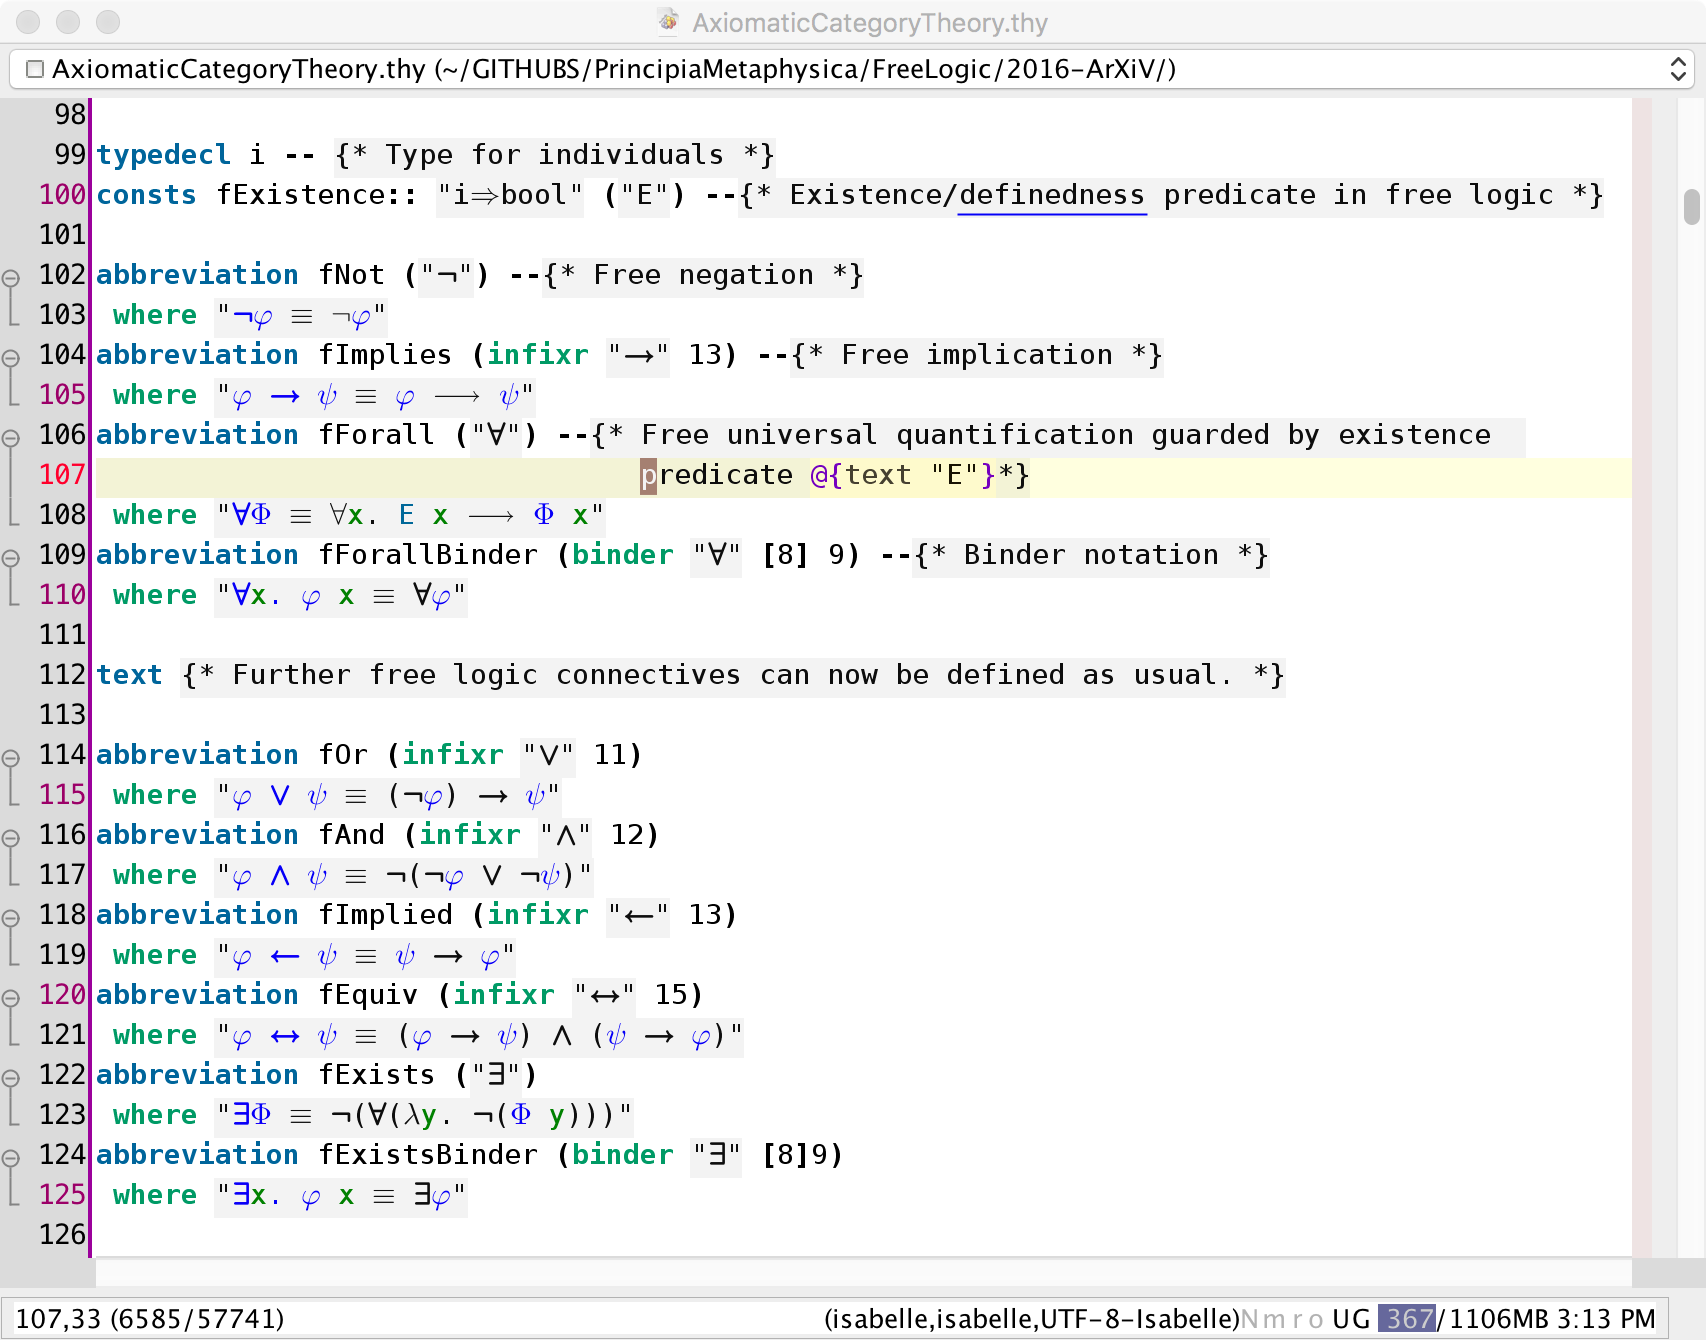
\includegraphics[width=\textwidth]{EmbeddingPic}
 \caption{Isabelle/HOL formalisation of $\FFOL$ in $\HOL$ \label{pic1}}
\end{figure}

\section{Shallow Semantical Embedding of $\FFOL$ in HOL}

The existence predicate $E$ is realized in the embedding as a $\HOL$
predicate $\hol{\ex}$ of type $\hol{ i\ar o}$; we assume that a
respective constant symbol is given in the signature of \HOL.  The raw domain $\hol{D}$ is simply
associated with the set of all objects of type $\hol{i}$, respectively
with the universal
predicate $\hol{\lambda X_i. T}$. Moreover, let
constant symbol $\hol{\star}$ of type $i$ be in the signature of
\HOL. We assume that $\hol{\|E \star\|^{M,g}=F}$ for all $\hol{M,g}$
i.e. that the element denoted by $\hol{\star}$ is not an element of
the domain of existing objects denoted by $\hol{\ex}$.

\begin{definition}[Embedding of $\FFOL$ in \HOL]
Given a formula $s \in \FFOL$. We map each language construct $s$ in the
signature of $\FFOL$ to a corresponding term $\map{s}$ of \HOL. This
mapping is defined as follows:

\begin{tabular}{lcll}
$\map{x}$    & := & $\hol{X_i}$ &for all $x\in \V$\\
$\map{f(t^1,\ldots,t^n)}$    & := & $\hol{(f \map{t^1} \ldots \map{t^n})}$  \quad
              & for all $n$-ary $f\in F$\\
 & & &  $\hol{f}$ has type $\hol{\underbrace{{i \ar
               \ldots  \ar i} \ar }_{n\geq o} i}$\\
%$\map{p}$    & := & $\hol{p_o}$ & for all $0$-ary $p\in \P$\\
$\map{s = t}$    & := & $\hol{\map{s} = \map{t}}$ \\
$\map{p(t^1,\ldots,t^n)}$    & := & $\hol{(p \map{t^1} \ldots \map{t^n})}$  \quad
             &  for all $n$-ary $p\in P$ \\ 
   & & & $\hol{p}$ has type $\hol{\underbrace{{i \ar
               \ldots  \ar i} \ar }_{n\geq o} o}$\\
$\map{\neg \varphi}$ & := &  $\hol{\neg\map{\varphi}}$  \\
$\map{\varphi \Impl \psi}$ & := &  $\hol{ \map{\varphi} \Impl \map{\psi}}$  \\
$\map{\forall x. s}$ & := &  $\hol{\forall X_i. \ex
                       X_i \Impl \map{s}}$   \\
$\map{\Descr x. s}$ & := &  $\hol{\textbf{IfThenElse}}$ \\
  & & \quad $\hol{(\exists x. \ex x \wedge \map{s} \wedge (\forall
      y. (\ex y \wedge ((\lambda X_i. \map{s}) y)) \Impl y = x))}$ \\
  & & \quad $\hol{ (\Descr  X_i. \map{s})}$ \\
  & & \quad $\hol{\star}$  \\
\end{tabular}
where $\hol{\textbf{IfThenElse}}$ is an abbreviation for the term
$\hol{\lam{S_o}\lam{X_i}\lam{Y_i}. \Descr Z_i. (S_o \wedge Z = X) \vee
(\neg S_o \wedge Z
= Y)}$.

Further connectives can be introduced as usual: $r \vee  s := \neg r
\Impl s$, $r \wedge  s := \neg (\neg r \vee \neg s)$, 
\end{definition}



Todo ... the embedding in Isabelle/HOL is depicted in 
figure \ref{pic1}


% In this framework partial and total functions are modelled as follows: 
% A function $f$ is total if and only if for all $x$ we have $\ex x \imp \ex(f x)$ 
% For partial functions $f$ we may have some $x$ such that $\ex x$ but not
%  $\ex(f x)$. A function $f$ is strict  if  and only if for all $x$
% we have $\ex(f x) \imp \ex x$.


\section{Exploring Axioms Systems for Category Theory}
In an exemplary theory exploration study, we have shown how Scott's
\cite{Scott79} axiom system for category theory can be derived from a
notion of partial monoids. These axioms systems are presented in Table \ref{axioms-sets-1}.

The stepwise evolution has been described in \cite{R58}. Below we
summarise these experiments.  However, first we describe some basic
modeling decisions for the technical encoding in Isabelle/HOL. The
Isabelle/HOL sources of our experiments are available at
\url{todo-sources}. Note that in these sources we did add neither the
definite description operator nor the designated undefined object
$\star$, since both were not required in our experiments.


\begin{table}[tp] \centering \normalsize
\begin{tabular}{ll}
\hline
\\
\multicolumn{2}{c}{Axioms Set I} \\
%\hline
\\
 $S_{i}$ & $\ex(x \comp y) \imp (\ex x \wedge \ex y)$ \\
 $E_{i}$ & $\ex(x \comp y) \limp (\ex x \wedge \ex y \wedge (\exists z. z \comp
         z \cong z \wedge x \comp z \cong x \wedge z \comp y \cong y))$ \\
 $A_{i}$ & $x\comp (y \comp z) \cong (x \comp y) \comp z$ \\
 $C_{i}$ & $\forall y. \exists i.  \id i \wedge i \comp y \cong y$ \\
 $D_{i}$ & $\forall x. \exists j.  \id j \wedge x \comp j \cong x$  \\
\\
\hline
\\
\multicolumn{2}{c}{Axioms Set II} \\
%\hline
\\
$S_{ii}$ & $\ex(x \comp y) \imp (\ex x \wedge \ex y) \wedge (\ex (\dom x) \imp \ex
        x) \wedge (\ex (\cod y) \imp \ex
        y)$ \\
 $E_{ii}$ & $\ex(x \comp y) \limp (\ex x \wedge \ex y \wedge (\exists z. z \comp
         z \cong z \wedge x \comp z \cong x \wedge z \comp y \cong y))$ \\
 $A_{ii}$ & $x\comp (y \comp z) \cong (x \comp y) \comp z$ \\
 $C_{ii}$ & $\ex y \imp (\id(\cod y) \wedge (\cod y) \comp y \cong y)$ \\
 $D_{ii}$ & $\ex x \imp (\id(\dom x) \wedge x \comp (\dom x) \cong x)$ \\
\\
\hline
\\
\multicolumn{2}{c}{Axioms Set III} \\
%\hline
\\
$S_{iii}$ & $\ex(x \comp y) \imp (\ex x \wedge \ex y) \wedge (\ex (\dom x) \imp \ex
        x) \wedge (\ex (\cod y) \imp \ex
        y)$ \\
 $E_{iii}$ & $\ex(x \comp y) \limp (\dom x \cong \cod y \wedge \ex (\cod y)))$ \\
 $A_{iii}$ & $x\comp (y \comp z) \cong (x \comp y) \comp z$ \\
 $C_{iii}$ & $\ex y \imp (\id(\cod y) \wedge (\cod y) \comp y \cong y)$ \\
 $D_{iii}$ & $\ex x \imp (\id(\dom x) \wedge x \comp (\dom x) \cong x)$ \\
\\
\hline
\\
\multicolumn{2}{c}{Axioms Set IV} \\
%\hline
\\
$S_{iv}$ & $\ex(x \comp y) \imp (\ex x \wedge \ex y) \wedge (\ex (\dom x) \imp \ex
        x) \wedge (\ex (\cod y) \imp \ex
        y)$ \\
 $E_{iv}$ & $\ex(x \comp y) \biimp (\dom x \cong \cod y \wedge \ex (\cod y)))$ \\
 $A_{iv}$ & $x\comp (y \comp z) \cong (x \comp y) \comp z$ \\
 $C_{iv}$ & $(\cod y) \comp y \cong y$ \\
 $D_{iv}$ & $x \comp (\dom x) \cong x$  \\
\\
\hline
\\
\multicolumn{2}{c}{Axioms Set V (Scott 79, \cite{Scott79})} \\
%\hline
\\
$S1$ & $\ex (\dom x) \imp \ex x$ \\
$S2$ & $\ex (\cod y) \imp \ex y$ \\
$S3$ & $\ex(x \comp y) \biimp \dom x \simeq \cod y$ \\
$S4$ & $x\comp (y \comp z) \cong (x \comp y) \comp z$ \\
$S5$ & $(\cod y) \comp y \cong y$ \\
$S6$ & $x \comp (\dom x) \cong x$  \\
\\
\hline
\end{tabular}
\caption{Stepwise evolution of Scott's \cite{Scott79} axiom
  system for category theory from partial monoids. The axiom names are
  motivated as follows: 
  $S$ stands for strictness, $E$ for existence, $A$ for associativity, $C$ for
  codomain, $D$ for Domain. The free variables $x$, $y$, $z$ range over
  the raw domain $D$. The quantifiers in Axiom Sets I and II are
  free logic quantifiers, that is, they range over the domain $E$ of
  existing objects. \label{axioms-sets-1}}
\end{table}





\subsection{Modeling of basic concepts}
Morphisms in the category are modeled as objects of type $\ti$. We introduce three partial functions, 
$\dom$ (domain), $\cod$ (codomain), and $\comp$ (morphism composition). 
Partiality of composition is handled exactly as expected: we generally may have 
non-existing compositions $x\comp y$ (i.e. $\neg(\ex(x\comp y))$) for some existing  
morphisms $x$ and $y$ (i.e. $\ex x$ and $\ex y$).

For composition $\comp$ we assume set-theoretical composition here (i.e., functional 
composition from right to left). This means that
\[(\cod x) \comp (x \comp (\dom x)) \kleq x\] 
and that 
\[(x \comp y)a \kleq x(y a) \quad \text{when}\quad
\dom x \exid \cod y\] 
The equality symbol $\kleq$ denotes Kleene equality and it
is defined as follows (where $=$ is identity on all objects, existing or non-existing, 
of type $\ti$):
\[x \kleq y \ddef (\ex x \vee \ex y) \imp x = y\]
Existing identity $\simeq$ is defined as:
\[x \simeq y \ddef \ex x \wedge \ex y \wedge  x = y\]

$\cong$ is an equivalence relation. $\simeq$, in contrast, is only symmetric and transitive, and lacks 
reflexivity. These observations are quickly confirmed by Isabelle.


Next, we define the identity morphism predicate $\id$ as follows: 

abbreviation I where \[\id i \ddef (\forall x. \ex(i \comp x) \imp i \comp
x \cong x) \wedge (\forall x. \ex(x \comp i) \imp x \comp i \cong x)\]

This definition was suggested by an exercise in \cite{FreydScedrov90}
on p.~4.  In earlier experiments we used a longer definition which can
be proved equivalent on the basis of the other axioms. For monoids,
where composition is total, $\id i$ means $i$ is a two-sided identity
— and such are unique. For categories the property is much weaker.
 

\subsection{Consistency}
The model finder Nitpick confirms consistency for all of the axiom
sets from Table \ref{axioms-sets-1}. For example, when asked to consider at least one defined and one undefined object, then
Nitpick generates for all cases the following model (called $M_1$ in the remainder):
$D=\{i_i,i_2\}$ and $E=\{i_1\}$;  $i_1\comp i_1$ is $i_1$,  and $i_2$
in all other cases; $\cod$ and $\dom$ are identity on $D$. Without constraining the request, Nitpick
generates an even simpler model (called $M_0$ in the remainder):
$D=\{i_i\}$ and $E=\emptyset$; $i_1\comp i_1$ is $i_1$; $\cod$ and
$\dom$ are identity on $D$. It is trivial to check that these models
indeed confirm the consistency of all axiom sets from Table \ref{axioms-sets-1}.

  % Constants:
   % codomain = (λx. _)(i⇩1 := i⇩1)
   %  op ⋅ = (λx. _)((i⇩1, i⇩1) := i⇩1)
   %  domain = (λx. _)(i⇩1 := i⇩1)
   %  E = (λx. _)(i⇩1 := False)


  % Constants:
  %   codomain = (λx. _)(i⇩1 := i⇩1, i⇩2 := i⇩2)
  %   op ⋅ = (λx. _)((i⇩1, i⇩1) := i⇩1, (i⇩1, i⇩2) := i⇩2, (i⇩2, i⇩1) := i⇩2, (i⇩2, i⇩2) := i⇩2)
  %   domain = (λx. _)(i⇩1 := i⇩1, i⇩2 := i⇩2)
  %   E = (λx. _)(i⇩1 := True, i⇩2 := False)



\subsection{Axioms Set I}
 Axioms Set I is our most basic axiom set for category theory generalizing the 
axioms for a monoid to a partial composition operation. Remember that a monoid is an 
algebraic structure $(S,\circ)$, where $\circ$ is a binary operator on set $S$, 
satisfying the following properties: 
$$
\begin{tabular}{ll}
Closure: & $ \forall a,b \in S.\ a \circ b \in S$ \\
Associativity: & $\forall a,b,c \in S.\ a \circ (b \circ c) = (a \circ b) \circ c$ \\
Identity: & $\exists id_S \in S. \forall a\in S.\ id_S\circ a = a = a \circ id_S$
\end{tabular}
$$

That is, a monoid is a semigroup with a two-sided identity element.

Axioms Set I generalises the notion of a monoid by introducing a partial, strict binary 
composition operation $\comp$. The existence of left and right identity elements is 
addressed in the last two axioms. The notions of $\dom$ (Domain) and
$\cod$ (Codomain)
abstract from their common meaning in the context of sets. In category theory we
work with just a single type of objects (the type $\ti$ of morphisms) and therefore 
identity morphisms are employed to suitably characterize their
meanings.

We can prove that the $i$ in axiom $C_i$ and the $j$ in axiom $D_i$
are unique. The proofs and the dependencies can be 
   found automatically by Sledgehammer.
$$  \forall y. \exists i. \id i \wedge i \comp y \cong y
\wedge (\forall j.d(\id j \wedge j \comp y \cong y) \imp i \cong j)
\quad 
    (\text{by } A_i, C_i, S_i) $$
$$ \forall x. \exists j. \id j \wedge x \comp j \cong x \wedge
(\forall i. (\id i \wedge x \comp i \cong x) \imp j \cong i) \quad   
    (\text{by }  A_i, D_i, S_i) $$

However, the $i$ and $j$ need not be equal. Using existential
variables $C$ and $D$, this can be encoded in
   our formalization as follows: 
 $$\exists C, D. (\forall y. \id (C y) \wedge (C y) \comp y \cong y)
 \wedge (\forall x. \id (D x) \wedge x \comp (D x) \cong x) \wedge
 D \not= C$$

The model finder Nitpick confirms that this formula is satisfiable:
e.g. choose domain $D=\{i_1,i_2\}$ and $E=\{i_2\}$; $i_2\comp i_2$ returns $i_2$,  and $i_1$
in all other cases; variable $D$ is identity on domain $D$, but $C$ maps both
$i_1$ and $i_2$ to $i_2$. 



\subsection{Axioms Set II}
Axioms Set II is developed from Axioms Set I by Skolemization of the
existentially quantified variables $i$ and $j$ in axioms $C_i$ and
$D_i$. We can argue semantically that every model of Axioms Set I has
such functions. Hence, we get a conservative extension of Axioms Set
I. This could be done for any theory with an $\forall x. \exists i$.-axiom. The strictness axiom $S$ is extended, so
that strictness is now also postulated for the new Skolem functions
$\dom$ and $\cod$. Note that the values of Skolem functions
outside $E$ can just be given by the identity function.

The left-to-right direction of existence axiom $E_{ii}$ is implied. 
  $$E(x \comp y) \imp (E x \wedge E y \wedge (\exists z. z \comp z
  \cong z \wedge x \comp z \cong x \wedge z\comp y \cong y)) \quad
  (\text{by } A_{ii}, C_{ii}, S_{ii})$$

Axioms $C_{ii}$ and $D_{ii}$, together with $S_{ii}$, show that
${\dom}$ and ${\cod}$ are total functions, as intended: 
$$E x \imp E(\dom x) \quad (\text{by } D_{ii}, S_{ii})$$
$$E x \imp E(\cod x) \quad (\text{by } C_{ii}, S_{ii}) $$

The proofs are found by Sledgehammer and verified in Isabelle/HOL. Using Sledgehammer we have also
shown that Axioms Set II implies Axioms Set I. Vice versa, Axioms Set I
also implies Axioms Set II. This can easily 
be shown by semantical means on the meta-level.

\subsection{Remark on the Experiments}
All proofs above and all proofs in the rest of this paper (unless
stated otherwise) have been obtained fully automatically with the
Sledgehammer tool in Isabelle/HOL. This tool interfaces to prominent
first-order automated theorem provers such as CVC4 \cite{CVC4}, Z3
\cite{Z3}, E \cite{E} and Spass \cite{Spass}.  Remotely, also
  provers such as Vampire \cite{Vampire}, or the higher-order provers
  Satallax \cite{Satallax} and LEO-II \cite{LEO} can be reached. For
  example, to prove axiom $E_{iii}$ from Axioms Set II, we have called
  Sledgehammer on all axioms of Axioms Set II. The provers then, via
  Sledgehammer, suggested to call trusted/verified tools in
  Isabelle/HOL with the exactly required dependencies they
  detected. With the provided dependency information the trusted tools
  in Isabelle/HOL were then able to reconstruct the external proofs on
  their own.  This way we obtain a verification of our claims in
  Isabelle/HOL, in which all the proofs have nevertheless been
  contributed by automated theorem provers.


\subsection{Axioms Set III}
In Axioms Set III the existence  axiom  $E_{ii}$ from Axioms Set II  is simplified by taking advantage of 
  the two new Skolem functions ${\dom}$ and $\cod$.

The left-to-right direction of existence axiom $E_{iii}$ is implied.
  $$E(x \comp y) \imp (\dom x \cong \cod y \wedge E(\cod y)) \quad  
    (\text{by } A_{iii}, C_{iii}, D_{iii}, S_{iii})$$

 Axioms Set II and Axioms Set III are equivalent; this has been
 confirmed by the automated theorem provers and verified in Isabelle/HOL.

\subsection{Axioms Set IV}
Axioms Set IV simplifies the axioms $C_{iii}$ and  $D_{iii}$ . However, as it turned 
 out, these simplifications also require the existence axiom $E_{iii}$ to be strengthened into
 an equivalence.

 Axioms Set III and Axioms Set IV are equivalent; this has been
 confirmed by the automated theorem provers and verified in
 Isabelle/HOL.

\subsection{Axioms Set V}
Axioms Set V has been proposed by Scott \cite{Scott79} in the 1970s. 
This set of axioms is equivalent to the axiom set presented by Freyd
and Scedrov in their textbook ``Categories, Allegories''
\cite{FreydScedrov90}, when encoded in free logic, corrected/adapted
and further simplified.  Their axiom set is technically flawed when
encoded in our given context. This issue has been detected by
automated theorem provers with the same technical infrastructure as
employed so far. See Section\ref{sec-freyd-scedrov} for more
details. 

 Axioms Set IV and Axioms Set V are equivalent; again, this has been
 confirmed by the automated theorem provers and verified in
 Isabelle/HOL.

 \section{Assessment of the Axiom System by Freyd and
   Scedrov} \label{sec-freyd-scedrov} In this section we study the
 axioms set of Freyd and Scedrov from their textbook ``Categories,
 Allegories'' \cite{FreydScedrov90}.  In Subsection
 \ref{subsec-freyd-scedrov-1} we show, that their axioms set,
 replicated in Table \ref{axioms-sets-2} as Axioms Set VI, becomes
 inconsistent in our free logic setting if we assume non-existing
 objects of type $i$, respectively, if we assume that the operations
 are non-total.


\begin{table} \centering \normalsize
\begin{tabular}{ll}
\hline
\\
\multicolumn{2}{c}{Axioms Set FS-I:  Freyd and Scedrov in original notation (with issues)} \\
%\hline
\\
  $A1$ &  $\ex(x \circ y) \longleftarrow (x\Box \cong \Box y)$ \\ 
  $A2a$ & $((\Box x)\Box) \cong \Box x$ \\ 
  $A2b$ & $\Box (x\Box) \cong \Box x$ \\ 
  $A3a$ & $(\Box x) \circ x \cong x$ \\ 
  $A3b$ & $x \circ (x\Box) \cong x$ \\ 
  $A4a$ & $\Box(x \circ y) \cong \Box(x \circ (\Box y))$ \\ 
  $A4b$ & $(x \circ y)\Box \cong ((x\Box) \circ y)\Box$ \\ 
  $A5$   & $x \circ (y \circ z) \cong  (x \circ y) \circ z$ \\
\\
\hline
\\
\multicolumn{2}{c}{Axioms Set FS-II: Freyd and Scedrov in our notation (with issues)} \\
%\hline
\\
  $A1$  & $\ex (x \comp y) \longleftrightarrow \dom x \cong \cod y$ \\
  $A2a$ & $\cod(\dom x) \cong \dom x$ \\  
  $A2b$ & $\dom(\cod y) \cong cod y$ \\  
  $A3a$  & $x \comp (\dom x) \cong x$ \\ 
  $A3b$ & $(\cod y) \comp y \cong y$ \\
  $A4a$ & $\dom(x \comp y) \cong \dom((\dom x) \comp y)$ \\ 
  $A4b$ & $\cod(x \comp y) \cong \cod(x \comp (\cod y))$ \\ 
  $A5$   & $x \comp (y \comp z) \cong  (x \comp y) \comp z$   \\
\\
\hline
\\
\multicolumn{2}{c}{Axioms Set VI: Freyd and Scedrov in our notation
  and corrected} \\
%\hline
\\
  $A1'$  & $\ex (x \comp y) \longleftrightarrow \dom x \simeq\cod y$ \\
  $A2a$ & $\cod(\dom x) \cong \dom x$ \\  
  $A2b$ & $\dom(\cod y) \cong cod y$ \\  
  $A3a$  & $x \comp (\dom x) \cong x$ \\ 
  $A3b$ & $(\cod y) \comp y \cong y$ \\
  $A4a$ & $\dom(x \comp y) \cong \dom((\dom x) \comp y)$ \\ 
  $A4b$ & $\cod(x \comp y) \cong \cod(x \comp (\cod y))$ \\ 
  $A5$   & $x \comp (y \comp z) \cong  (x \comp y) \comp z$   \\
\\
\hline
\end{tabular}
\caption{The axioms set of Freyd and Scedrov in their and our
  notation, together with a proposed correction.\label{axioms-sets-2}}
\end{table}


 Note, however, that the free variables in this first study range over
 the existing and non-existing objects in domain $D$. One may argue,
 that this is not the intention of Freyd and
 Scedrov. Therefore, we add a second study in Subsection
 \ref{subsec-freyd-scedrov-2}, in which we restrict the
 variables to range only over existing objects in $E$. However, also in this case
 the axiom system of Freyd and Scedrov remains unsatisfactory. Now it
 turns out incomplete, 
 since strictness conditions/axioms are required which are not mentioned in
 the textbook.

  Freyd and Scedrov employ a different notation for $\dom x$ and $\cod
 x$. They denote these operations by $\Box x$ 
  and $x\Box$. Moreover, they employ diagrammatic composition $(f \circ
  g) x \cong g(f x)$ (functional composition from left to right) instead of the set-theoretic 
  definition $(f \comp g) x \cong f(g x)$ (functional composition from right to left) used so far.
  We leave it to the reader to verify that their Axioms
  Set VI corresponds to Axioms
  Set VII modulo an appropriate conversion of notation.\footnote{A recipe for 
  this translation is as follows: (i) replace all $x \circ y$ by
  $y \comp x$, (ii) rename the variables to get them again in alphabetical order,
(iii) replace $\varphi\Box$ by $\cod \varphi$ and $\Box\varphi$  by $dom \varphi$, and finally
(iv) replace $\cod y \cong \dom x$ (resp. $\cod y \simeq \dom x$) 
   by $\dom x \cong \cod y$ (resp. $\dom x \simeq \cod y$).}

\subsection{Constricted Inconsistency in Free Logic Setting} \label{subsec-freyd-scedrov-1}
  A main difference in the system by Freyd and Scedrov to our Axiom
  Set V from Table \ref{axioms-sets-1} concerns
  axiom $S3$ respectively $A1$. Namely, instead of the non-reflexive
  existing identity $\simeq$, they use Kleene 
  equality $\cong$, cf. definition 1.11 on page 3 of \cite{FreydScedrov90}.\footnote{Def. 1.11 in Freyd 
  Scedrov: ``The ordinary equality sign $=$ [i.e., our $\cong$] will be used in the
  symmetric sense, to wit: if either side is defined then so is the other and they are equal. \ldots''} 
  The difference seems minor, but in our free logic setting it has the effect to cause the mentioned
  constricted inconsistency issue. This could perhaps be an oversight, or it could indicate
  that Freyd and Scedrov actually mean the Axioms Set VIII below (where the variables in the axioms range 
  over defined objects only). However, in Axioms Set VIII we had to (re-)introduce explicit 
  strictness conditions to ensure equivalence to the Axiom Set V by
  Scott.

  The (constricted) inconsistency of Axioms Set FS-I, respectively
  Axiom Set FS-II, from Table \ref{axioms-sets-2} has been 
  detected first by the model finder Nitpick. When we asked Nitpick to
  generate a model with at least one non-existing object, it claimed
  that there is no such model. However, a model can still be
  constructed if we do not make any assumptions about non-existing
  objects. In fact, the model presented by Nitpick for this case
  consists of a single, existing morphism.

However, one can see directly that Axiom $A1$ is problematic
as written: If $x$ and $y$ are undefined, then
(presumably) $\dom x$ and $\cod y$ are undefined as
well, and by the definition of Kleene equality, $\dom x \cong \cod
  y$. $A1$ stipulates that $x \comp y$ should be defined in
this case, which appears unintended.

As we will demonstrate now, the consequences of this version of the axiom are
even stronger. It implies that \emph{all} objects are defined,
that is, composition (as well as $\dom$ and $\cod$) become total operations.
The theory described by these axioms ``collapses'' to the theory of
monoids: If all objects are defined, then one can conclude from $A1$ that 
$\dom x \cong \dom y$ (resp.~$\dom x \cong \cod y$) and $\cod x \cong \cod y$), 
and according to 1.14 of \cite{FreydScedrov90}, 
the category reduces to a monoid provided that it is not empty.

In fact, the automated theorem provers, via Sledgehammer, quickly
prove falsity from Axioms Set FS-II (or FS-I) when assuming a 
 non-existing object of type $i$:
$$(\exists x. \neg E x) \imp False$$

The provers identify the axioms $A1$,
 $A2a$ and $A3a$ to cause the problem under this assumption. A
 human-intuitive proof argument is as follows:
 
 Let $a\in D$ be an undefined object, that is, assume $¬E a$.  By
 instantiating axiom $A3a$ with $a$ we have $a \comp (\dom a) \cong a$.  From
 this and definition of $\cong$ we know that $a \comp (\dom a)$ is not
 defined. This is easy to see, since if $a \comp (\dom a)$ were defined, we
 also had that $a$ is defined, which is not the case by assumption.
  Hence, $\neg E (a \comp (\dom a)$.
Next, we instantiate $A1$ with $a$ and $\dom a$ to obtain
   $E(a \comp (\dom a)) \biimp \dom a \cong \cod(\dom a)$. Moreover,
   by instantiating $A2a$ with $a$ we obtain $\cod(\dom a) \cong dom a$,
   which we use (modulo symmetry and transitivity of $\cong$) to
   rewrite the former result into 
   $E(a \comp (\dom a)) \biimp \dom a \cong \dom a$. By reflexivity of
   $\cong$ we thus get $E(a \comp (\dom a))$, i.e. that $a \comp
   (\dom a)$ is defined, which contradicts $\neg E (a \comp (\dom
   a)$. $\Box$

As a corollary from the above constricted inconsistency result we get that all  must be
defined: $\forall x. E x$




% We also
%  show
%  that there is a simple fix to that issue, namely to replacement of
%  the occurence of Kleene equality in one axiom by  

% We have modified the axioms of \cite{FreydScedrov90} by
% replacing the original Kleene equality $\cong$ in their axiom $S3$ by
% the non-reflexive, existing identity $\simeq$. Note that the modified
% axiom $S3$ is equivalent to $E_{iv}$.\marginpar{Check again} 

%  this study we assume 

% However, this time we restrict 
% the free variables in their system to range over existing objects only. By employing the free logic 
% universal quantifier @{text "❙∀"} we thus modify Axiom Set VII as follows:


\begin{table} \centering \normalsize
\begin{tabular}{ll}
\\
\hline
\\
\multicolumn{2}{c}{Freyd and Scedrov in our notation (corrected and
  reduced I)} \\
%\hline
\\
  $B1'$  & $\ex (x \comp y) \longleftrightarrow \dom x \simeq\cod y$ \\
  $B3a$  & $x \comp (\dom x) \cong x$ \\ 
  $B3b$ & $(\cod y) \comp y \cong y$ \\
  $B4a$ & $\dom(x \comp y) \cong \dom((\dom x) \comp y)$ \\ 
  $B4b$ & $\cod(x \comp y) \cong \cod(x \comp (\cod y))$ \\ 
  $B5$   & $x \comp (y \comp z) \cong  (x \comp y) \comp z$   \\
\\
\hline
\\
\multicolumn{2}{c}{Freyd and Scedrov in our notation (corrected and
  reduced II)} \\
%\hline
\\
  $B1'$  & $\ex (x \comp y) \longleftrightarrow \dom x \simeq\cod y$ \\
  $B2a$ & $\cod(\dom x) \cong \dom x$ \\  
  $B2b$ & $\dom(\cod y) \cong cod y$ \\  
  $B3a$  & $x \comp (\dom x) \cong x$ \\ 
  $B3b$ & $(\cod y) \comp y \cong y$ \\
  $B5$   & $x \comp (y \comp z) \cong  (x \comp y) \comp z$   \\
\\
\hline
\\
\multicolumn{2}{c}{Freyd and Scedrov in our notation (corrected and
  reduced III)} \\
%\hline
\\
 $S^1_{v}$ & $\ex (\dom x) \imp \ex x$ \\
  $S^2_{v}$ & $\ex (\cod y) \imp \ex y$ \\
  $B1'$  & $\ex (x \comp y) \longleftrightarrow \dom x \simeq\cod y$ \\
  $B3a$  & $x \comp (\dom x) \cong x$ \\ 
  $B3b$ & $(\cod y) \comp y \cong y$ \\
  $B5$   & $x \comp (y \comp z) \cong  (x \comp y) \comp z$   \\
\\
\hline
\end{tabular}
\caption{Bla}
\end{table}


\subsection{Missing Strictness Axioms in Alternative Setting} \label{subsec-freyd-scedrov-2}

\section{Conclusion}
\ldots todo

\begin{acknowledgements}
DFG projects \ldots todo
\end{acknowledgements}

% BibTeX users please use one of
%\bibliographystyle{spbasic}      % basic style, author-year citations
\bibliographystyle{spmpsci}      % mathematics and physical sciences
%\bibliographystyle{spphys}       % APS-like style for physics
\bibliography{bibliography}   % name your BibTeX data base

% % Non-BibTeX users please use
% \begin{thebibliography}{}
% %
% % and use \bibitem to create references. Consult the Instructions
% % for authors for reference list style.
% %
% \bibitem{RefJ}
% % Format for Journal Reference
% Author, Article title, Journal, Volume, page numbers (year)
% % Format for books
% \bibitem{RefB}
% Author, Book title, page numbers. Publisher, place (year)
% % etc
% \end{thebibliography}

\end{document}
% end of file template.tex

